%%%%%%%%%%%%%%%%%%%%%%%%%%%%%%%%%%%%%%%%%
% Beamer Presentation
% LaTeX Template
% Version 1.0 (10/11/12)
%
% This template has been downloaded from:
% http://www.LaTeXTemplates.com
%
% License:
% CC BY-NC-SA 3.0 (http://creativecommons.org/licenses/by-nc-sa/3.0/)
%
%%%%%%%%%%%%%%%%%%%%%%%%%%%%%%%%%%%%%%%%%

%----------------------------------------------------------------------------------------
%	PACKAGES AND THEMES
%----------------------------------------------------------------------------------------

\documentclass{beamer}

\mode<presentation> {

% The Beamer class comes with a number of default slide themes
% which change the colors and layouts of slides. Below this is a list
% of all the themes, uncomment each in turn to see what they look like.

%\usetheme{default}
%\usetheme{AnnArbor}
%\usetheme{Antibes}
%\usetheme{Bergen}
%\usetheme{Berkeley}
%\usetheme{Berlin}
%\usetheme{Boadilla}
%\usetheme{CambridgeUS}
%\usetheme{Copenhagen}
%\usetheme{Darmstadt}
%\usetheme{Dresden}
%\usetheme{Frankfurt}
%\usetheme{Goettingen}
%\usetheme{Hannover}
%\usetheme{Ilmenau}
%\usetheme{JuanLesPins}
%\usetheme{Luebeck}
%\usetheme{Madrid}
%\usetheme{Malmoe}
%\usetheme{Marburg}
\usetheme{Montpellier}
%\usetheme{PaloAlto}
%\usetheme{Pittsburgh}
%\usetheme{Rochester}
%\usetheme{Singapore}
%\usetheme{Szeged}
%\usetheme{Warsaw}

% As well as themes, the Beamer class has a number of color themes
% for any slide theme. Uncomment each of these in turn to see how it
% changes the colors of your current slide theme.

%\usecolortheme{albatross}
%\usecolortheme{beaver}
%\usecolortheme{beetle}
%\usecolortheme{crane}
%\usecolortheme{dolphin}
%\usecolortheme{dove} %this seems cool
%\usecolortheme{fly}
%\usecolortheme{lily}
%\usecolortheme{orchid} %this is original
\usecolortheme{rose} % this one is also ok, maybe #1
%\usecolortheme{seagull}
%\usecolortheme{seahorse}
%\usecolortheme{whale}
%\usecolortheme{wolverine}

%\setbeamertemplate{footline} % To remove the footer line in all slides uncomment this line
%\setbeamertemplate{footline}[page number] % To replace the footer line in all slides with a simple slide count uncomment this line

\setbeamertemplate{navigation symbols}{} % To remove the navigation symbols from the bottom of all slides uncomment this line
}

\usepackage{booktabs} % Allows the use of \toprule, \midrule and \bottomrule in tables
\usepackage[utf8]{inputenc}
\usepackage[dvipdfmx]{graphicx} 
\usepackage{bmpsize}
\usepackage{grffile}
%----------------------------------------------------------------------------------------
%	TITLE PAGE
%----------------------------------------------------------------------------------------

\title[BFP Tools]{Profiling with BPF tools} % The short title appears at the bottom of every slide, the full title is only on the title page

\author{Piotr Wieleba} % Your name
\institute[DataArt] % Your institution as it will appear on the bottom of every slide, may be shorthand to save space
{
DataArt\\ % Your institution for the title page
\medskip
\textit{piotr.wieleba@dataart.com} % Your email address
}
\date{\today} % Date, can be changed to a custom date

\begin{document}

\begin{frame}
\titlepage % Print the title page as the first slide
\end{frame}

%\begin{frame}
%\frametitle{Hello}
%\begin{itemize}
%\item<1-> Work in Java/JVM centric technologies for over 11 years
%\item<2-> Currently in DataArt Lublin
%\item<3-> Worked in different domains (education, health care, finance, retail)
%\item<4-> Mostly programming but also been doing a little bit of SRE
%\end{itemize}
%\end{frame}

%----------------------------------------------------------------------------------------
%	PRESENTATION SLIDES
%----------------------------------------------------------------------------------------

\section{Motivation}
\begin{frame}
    \centering
		\huge Why this subject?
\end{frame}

\begin{frame}
  \begin{figure}
    \centering
		\noindent\makebox[\textwidth]{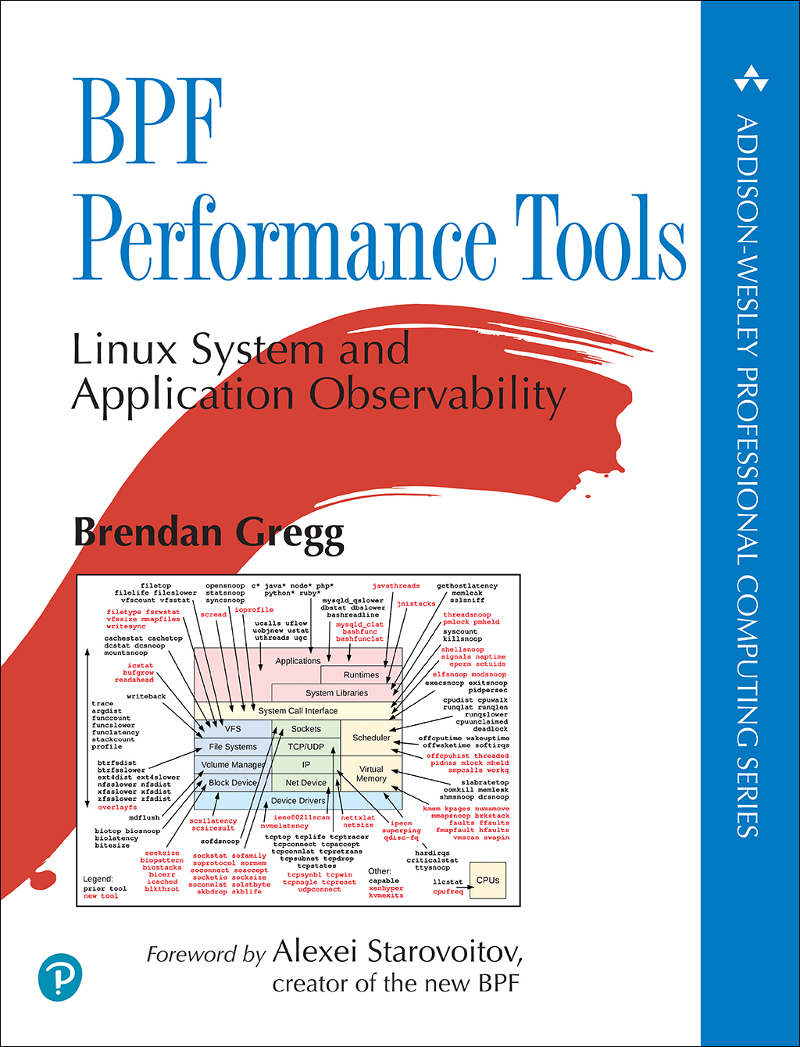
\includegraphics[scale=0.4]{cover}}
  \end{figure}
\end{frame}

\begin{frame}
  \begin{figure}
    \centering
    \noindent\makebox[\textwidth]{
\includegraphics[width=\paperwidth]{twitter_1}}
  \end{figure}
\end{frame}

%------------------------------------------------
\section{Introduction} % Sections can be created in order to organize your presentation into discrete blocks, all sections and subsections are automatically printed in the table of contents as an overview of the talk
%------------------------------------------------
\subsection{Basic Terms}

\begin{frame}
  \begin{block}{Tracing}
		\begin{LARGE}
			\begin{itemize}
				\item<+-> Event-based recording.  
				\item<+-> Can show periodicaly updated, statistics.
				\item<+-> Tracers are: \emph{strace}, \emph{top}, \emph{tcpdump}. 
			\end{itemize}
		\end{LARGE}
  \end{block}
\end{frame}


\begin{frame}
  \begin{block}{Snooping}
    \begin{itemize}
      \item \LARGE \emph{snoop = tracer}
    \end{itemize}
  \end{block}
\end{frame}


\begin{frame}
  \begin{block}{Sampling/Profiling}
		\begin{Large}
			\begin{itemize}
				\item<+-> Analyze sub-set of all events
				\item<+-> Performance overhead can be lower than for tracers
				\item<+-> Samples can be taken once every n miliseconds 
			\end{itemize}
		\end{Large}
  \end{block} 
\end{frame}


\begin{frame}
  \begin{block}{Observability}
		\begin{Large}
			\begin{itemize}
				\item<+-> Reasoning about the system through observation
				\item<+-> Observability tools including tracers, samplers
				\item<+-> Benchmarks are not observability tools
			\end{itemize}
		\end{Large}
  \end{block} 
\end{frame}


\subsection{BPF} % A subsection can be created just before a set of slides with a common theme to further break down your presentation into chunks

\begin{frame}
\frametitle{History}
		\begin{Large}
			\begin{itemize}
				\item<1-> Original BPF (Berkeley Packet Filter)
				\item<2-> eBPF ~2014 Alexei Starovoitov
				\item<3-> Nowdays BPF means actually eBPF
			\end{itemize}
		\end{Large}
\end{frame}

\begin{frame}
  \frametitle{How BPF looks like?}
  \begin{itemize}
    \item<1-> BPF =  bytecode similar to assembly language
    \item<2-> Designed to be emmited by higher level tools
    \item<3-> {\scriptsize \texttt{\# bpftrace -e 'tracepoint:syscalls:sys\_enter\_exec* \{ @[comm, pid]=count();\}' }}
		\begin{block}{\scriptsize \texttt{\# bpftool prog dump xlated id 4}}
      {\texttt 
			 0: (b7) r1 = 0

			 1: (7b) *(u64 *)(r10 -8) = r1

			 2: (7b) *(u64 *)(r10 -16) = r1

			 3: (bf) r1 = r10

			 4: (07) r1 += -16

			 5: (b7) r2 = 16

			 6: (85) call bpf\_get\_current\_comm\#119536
			 
			 ................
		  }
      \end{block}
  \end{itemize}
\end{frame}

\begin{frame}
  \frametitle{What makes BPF based tools sufficient for analysis in production}
	\begin{Large}
  \begin{itemize}
		\item<+-> Build-in into kernel
    \item<+-> Efficient 
		\item<+-> Production safe 
	\end{itemize}
	\end{Large}
\end{frame}

\subsection{Instrumentation}

\begin{frame}
  \frametitle{Dynamic Instrumentation kprobes}

	\begin{Large}
  \begin{itemize}
    \item<1-> Kprobes can instrument any kernel function
		\item<2-> Kretprobe allows checking ret vals
		\item<3-> In bpftrace kprobes starts with 'kprobe:' or simple 'k:'
    \item<4-> Breakepoint instruction int3 or jmp is set in place of target function address and is removed when no longer needed
    \item<5-> {\scriptsize \texttt{\# bpftrace -l 'kprobe:*'}}
	\end{itemize}	
\end{Large}
\end{frame}

\begin{frame}
  \frametitle{Dynamic Instrumentation uprobes}
	\begin{Large}
  \begin{itemize}
    \item<1-> Uprobes are probes for user-space processes
		\item<2-> Uretprobe
		\item<3-> In bpftrace uprobes starts with 'uprobe:' or simple 'u:'
		\item<4-> Can be use to instrument libraries and binary
    \item<5-> {\scriptsize \texttt{\# bpftrace -l 'uprobe:/lib/x86\_64-linux-gnu/libc.so.6' }}
	\end{itemize}	
\end{Large}
\end{frame}


\begin{frame}
	\frametitle{Demo}
	\begin{Huge}
  \begin{itemize}
    \item<1-> INT3
	\end{itemize}	
\end{Huge}
\end{frame}

\begin{frame}
  \frametitle{Static Instrumentation}
	\begin{itemize}
	  \item<1-> Dynamic instrumentation can instrument functions. Name of the function can change or can be inlined so script can stop working with new version of the library/kernel
		\item<2-> Static instrumentation rely on stable event names not function names
		\item<3-> Downside is that SI is harder to maintenance
		\item<4-> Static kernel instrumentation $\Rightarrow$ tracepoints
		\item<5-> Static user-space instrumentation $\Rightarrow$ USDT user-level statically defined tracing
	\end{itemize}
\end{frame}

\begin{frame}
  \frametitle{Cost}
	\begin{Large}
		\begin{itemize}
			\item<+-> Tracepoint introduce tiny time penalty and space penalty
			\item<+-> Dynamic probes doesn't introduce cost when off
			\item<+-> Raw tracepoints = faster version of normal tracepoints
		\end{itemize}
	\end{Large}
\end{frame}


%------------------------------------------------
\subsection{FrontEnd tools for BPF}
\begin{frame}
  \frametitle{BCC (BPF Compiler Collection)}
	\begin{Large}
  \begin{itemize}
    \item<+-> BCC allows to write BPF kernel in C and user interface in Python, Lua or C++
    \item<+-> Instalation provides over 70 ready to use performance analysis tools
    \item<+-> No need to write BCC code by yourself
    \item<+-> /usr/share/bcc/tools
  \end{itemize}
\end{Large}
\end{frame}

\begin{frame}
  \begin{figure}
    \centering
		\noindent\makebox[\textwidth]{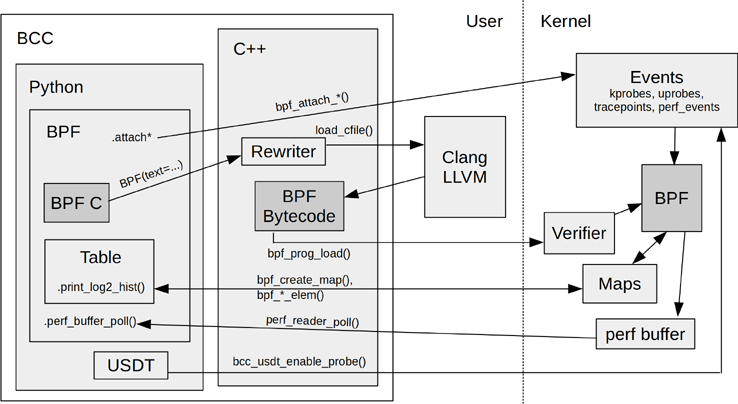
\includegraphics[scale=0.4]{bcc_internals}}
  \end{figure}
\end{frame}



\begin{frame}
  \frametitle{bpftrace}
	\begin{Large}
  \begin{itemize}
    \item<+-> New frontend tool
    \item<+-> Provide AWK like language to write very specific analytic tools often called oneliners
    \item<+-> More complicated tools can be written as a '.bt' scripts
  \end{itemize}
\end{Large}
\end{frame}

\begin{frame}
  \begin{figure}
    \centering
		\noindent\makebox[\textwidth]{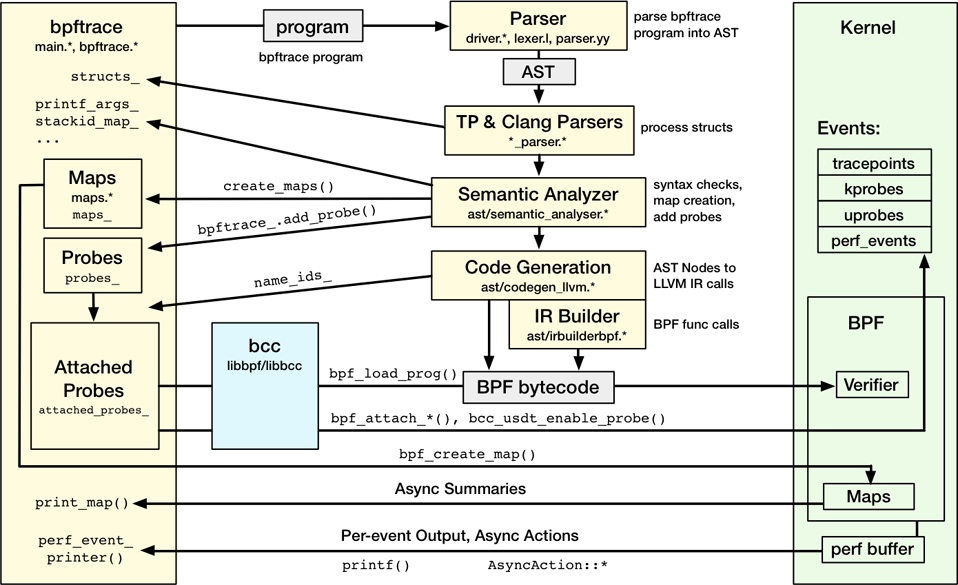
\includegraphics[scale=0.4]{bpftrace_internals.jpg}}
  \end{figure}
\end{frame}


\begin{frame}
  \begin{figure}
    \centering
    \noindent\makebox[\textwidth]{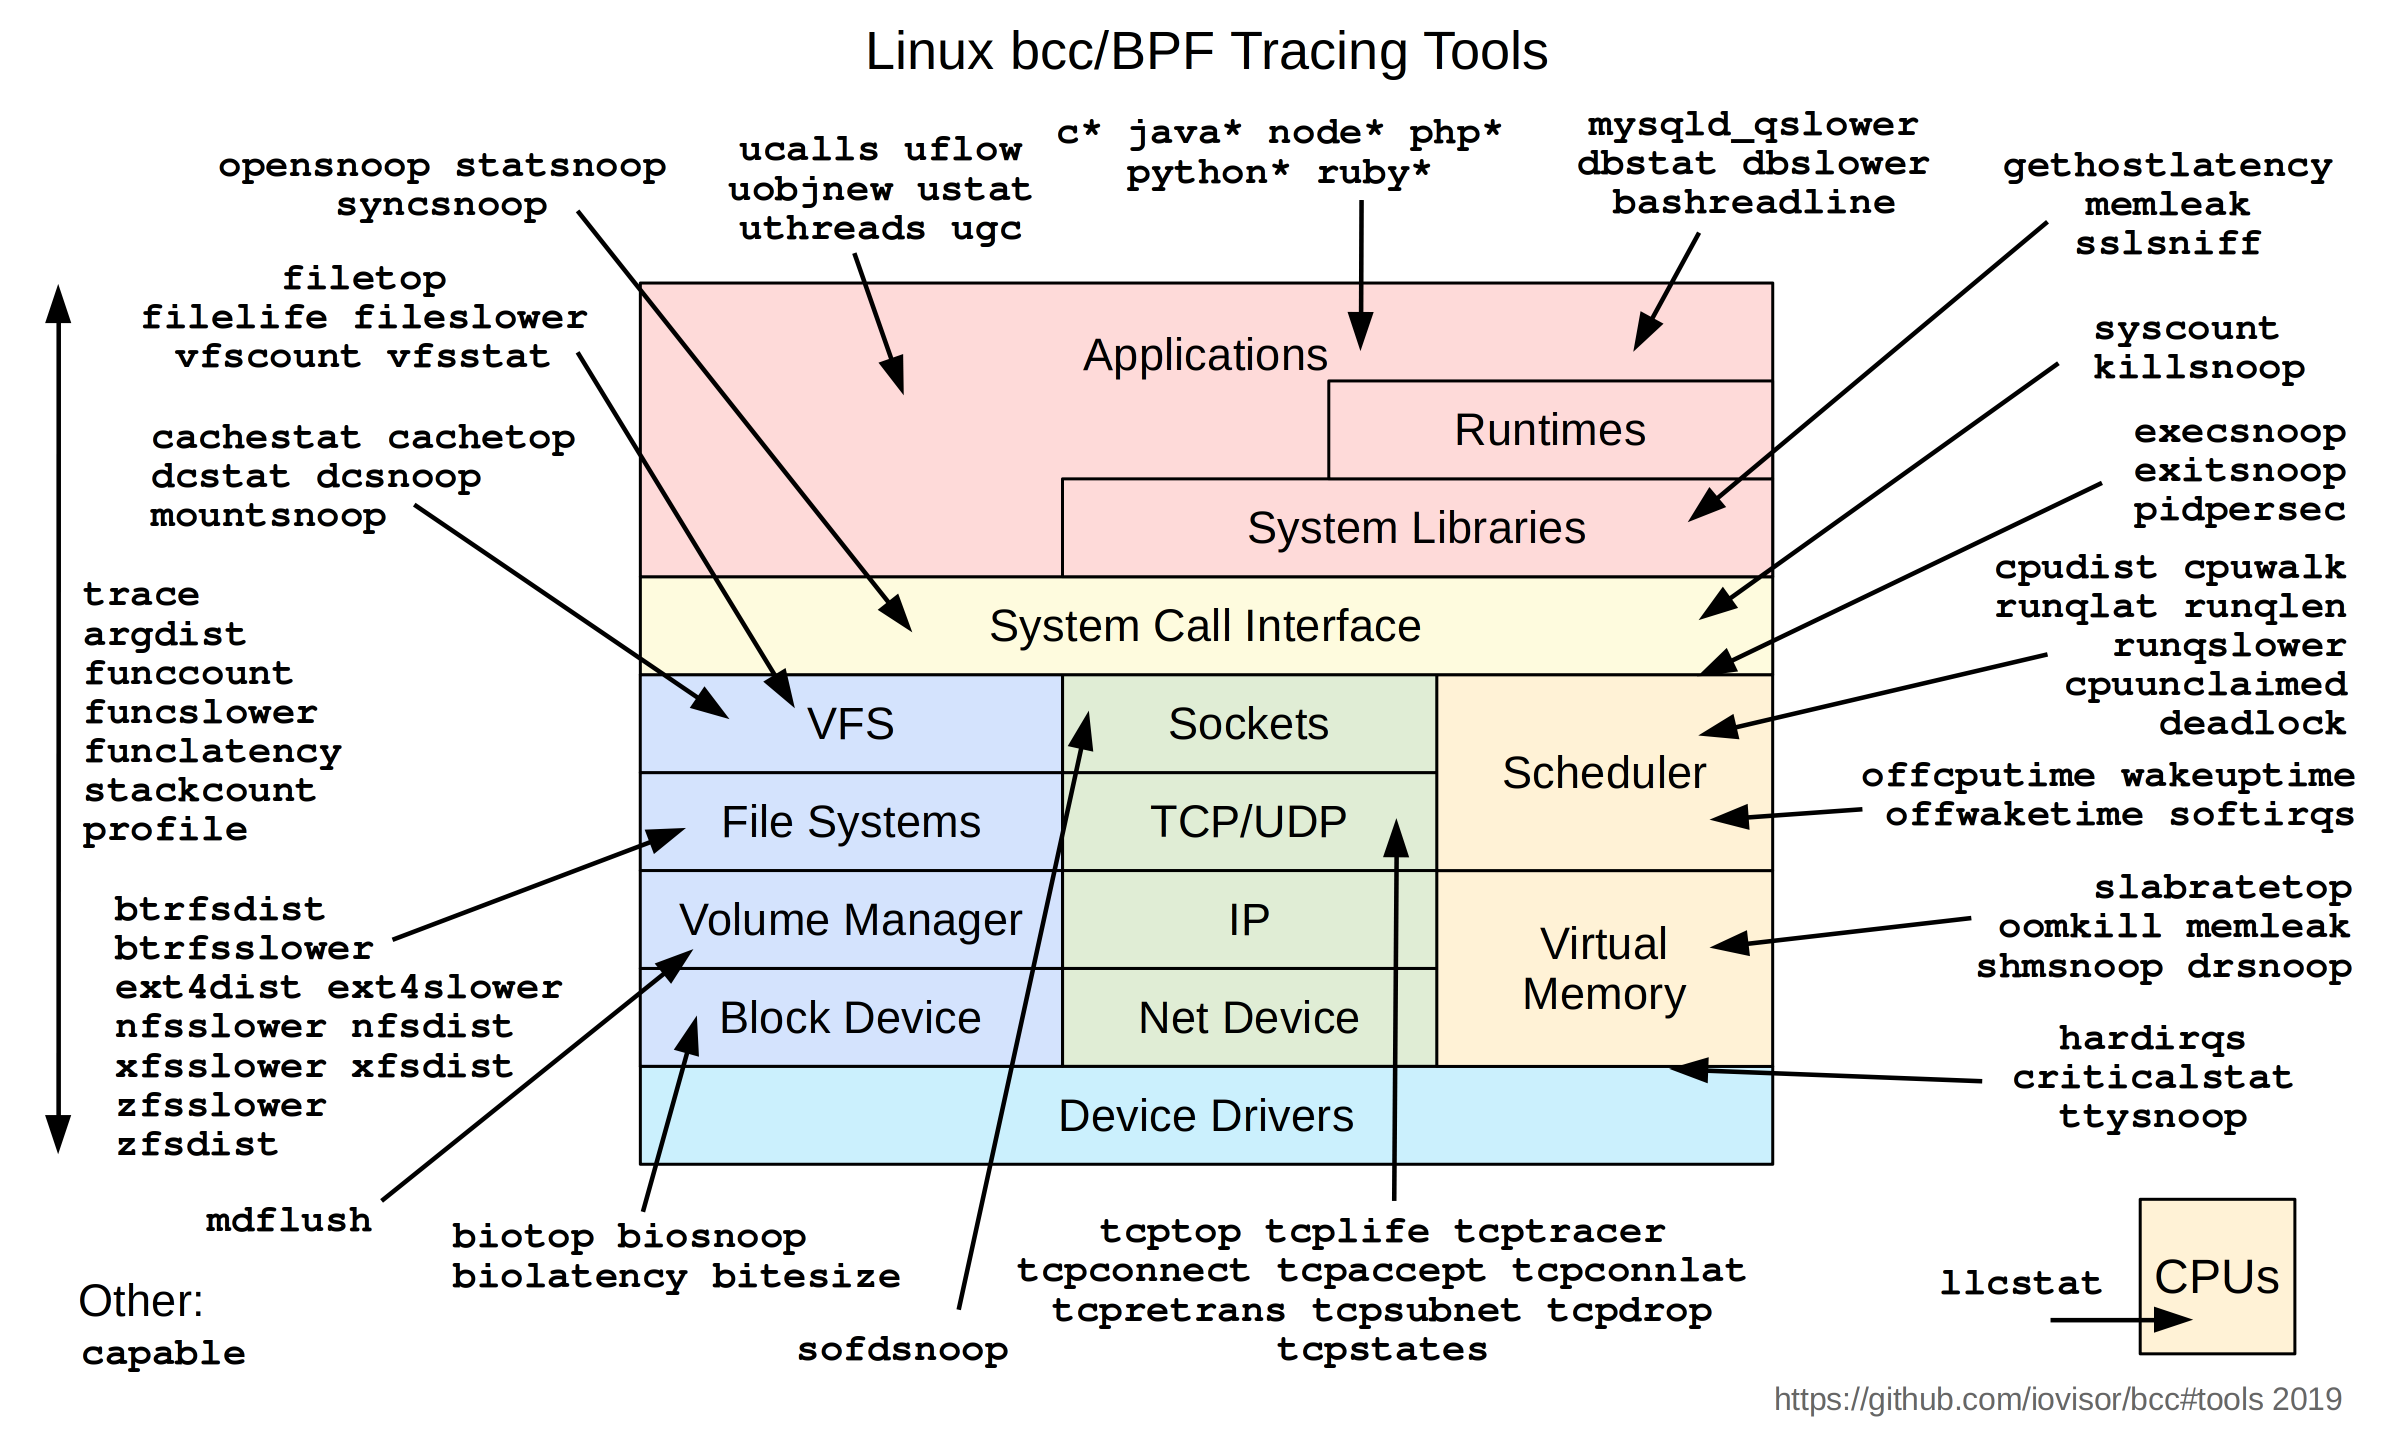
\includegraphics[width=\paperwidth]{bcc_tracing_tools_2019}}
  \end{figure}
\end{frame}


%------------------------------------------------
\section{Demo}
%------------------------------------------------

\begin{Large}


\subsection{CPU}

\begin{frame}
	\begin{itemize}
		\item<+-> cpuwalk
		\item<+-> cpudist
		\item<+-> runqlen
		\item<+-> runqlat
		\item<+-> runqslower
		\item<+-> execsnoop
		\item<+-> exitsnoop
		\item<+-> offcputime
	\end{itemize}
\end{frame}

\subsection{VFS}
\begin{frame}
	\begin{itemize}
		\item<+-> opensnoop
		\item<+-> statsnoop 
		\item<+-> syncsnoop
		\item<+-> vfsstat
		\item<+-> vfscount
		\item<+-> vfssize.bt
		\item<+-> filetop
		\item<+-> filelife
		\item<+-> fileslower
		\item<+-> mountsnoop
	\end{itemize}
\end{frame}

\subsection{IO}
\begin{frame}
	\begin{itemize}
		\item<+-> biolatency
		\item<+-> iostat 
		\item<+-> biosnoop.bt
		\item<+-> bitesize
	\end{itemize}
\end{frame}

\subsection{Network}
\begin{frame}
	\begin{itemize}
		\item<+-> gethostlatency
		\item<+-> tcpconlat 
	\end{itemize}
\end{frame}

\subsection{Memory}
\begin{frame}
	\begin{itemize}
		\item<+-> memleak (System Libraries)
		\item<+-> mmapsnoop (System Call Interface) 
		\item<+-> brkstack (System Call Interface)
		\item<+-> vmscan (Virtual Memory)
		\item<+-> shmsnoop (shared memory syscalls)
		\item<+-> drsnoop (direct reclaim)
		\item<+-> oomkill (Virtual Memory)
	\end{itemize}
\end{frame}

\end{Large}

\subsection{oneliners}
\begin{frame}[fragile] % Need to use the fragile option when verbatim is used in the slide
\frametitle{Example Oneliners}
\begin{example}[Open File]
\begin{verbatim}
# bpftrace -e 'tracepoint:syscalls:sys_enter_open {
  printf("%d %s %s\n", pid, comm, str(args->filename));
}'
\end{verbatim}
\end{example}
\end{frame}


\begin{frame}[fragile] % Need to use the fragile option when verbatim is used in the slide
\frametitle{Example Oneliners}
\begin{example}[Number of times when process open a file]
\begin{verbatim}
# bpftrace -e 't:syscalls:sys_enter_open { 
  @[comm, str(args->filename)] = count();
}'
\end{verbatim}
\end{example}
\end{frame}

\begin{frame}
\frametitle{References}
\footnotesize{
\begin{thebibliography}{99} % Beamer does not support BibTeX so references must be inserted manually as below
\bibitem[Gregg, 2020]{p1} Brendan Gregg (2020)
\newblock BPF Performance Tools
\newblock Linux System and Application Observability
\bibitem[iovisor]{p1} \url{https://github.com/iovisor/bcc}
\end{thebibliography}
}
\end{frame}

%------------------------------------------------

\begin{frame}
\Huge{\centerline{The End}}
\end{frame}

%----------------------------------------------------------------------------------------

\end{document} 
